
The most common way of using CMake is via the command-line interface (CLI). CLIs exist in virtually every environment, thus, learning to use CMake in a CLI is essential. In this section, we are going to learn how to perform the most basic CMake operations using the CLI.

Interactions with the CMake CLI can be done by issuing the cmake command in your operating system's terminal, assuming that CMake is installed and the cmake executable is included in your system's PATH variable (or equivalent). You can verify that by issuing cmake in your terminal without any parameters, as shown in the following figure:

\begin{center}
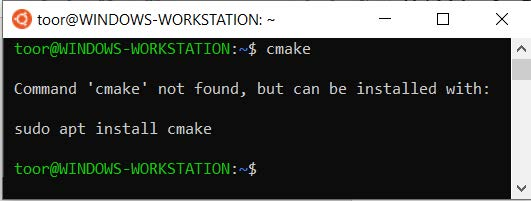
\includegraphics[width=1.\textwidth]{content/1/chapter2/images/1.jpg}\\
Figure 2.1 – Invoking the cmake command
\end{center}

If your terminal is complaining about a missing command, then you should either install CMake (explained in Chapter 1, Kickstarting CMake) or make it discoverable by adding it to your system's PATH variable. Consult your operating system's guide about how to add a path to the system's PATH variable.

After installing CMake and adding it to the PATH variable (if required), you should test whether CMake is usable. The most basic command you can execute in the command line is cmake -{}-version, which allows you to check CMake's version.

\begin{center}
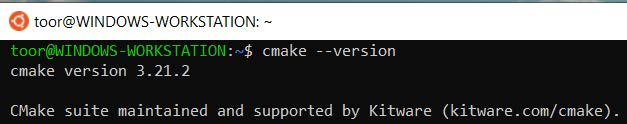
\includegraphics[width=1.\textwidth]{content/1/chapter2/images/2.jpg}\\
Figure 2.2 – Checking CMake's version in the terminal
\end{center}

CMake will output a version string in the form of cmake version <maj.min.rev>. You should see an output that contains the version number of CMake you've installed on your system.

\begin{tcolorbox}[colback=webgreen!5!white,colframe=webgreen!75!black,title=Note]
If the version does not match with the installed one, then you probably have multiple installations of CMake on your system. Since this book contains examples written for CMake version 3.21 and above, it is recommended to have that issue fixed before going any further.
\end{tcolorbox}

After installing CMake, you should install your build system and compiler as well. For Debian-like operating systems (for example, Debian and Ubuntu), this can be easily done by issuing the sudo apt install build-essential command. This package essentially contains gcc, g++, and make.

The CLI usage will be illustrated in the Ubuntu 20.04 environment. Apart from the minor edge cases, the usage is the same in other environments as well. Those edge cases will be mentioned as we go on.

\subsubsubsection{2.2.1\hspace{0.2cm}Learning the basics of the CMake CLI}

The three basic things you should learn about using the CMake CLI are listed here:

\begin{itemize}
\item 
Configuring a CMake project

\item 
Building a CMake project

\item 
Installing a CMake project
\end{itemize}

After learning the basics, you will be able to build and install any CMake project of your choice. Let's get started with configuring.

\hspace*{\fill} \\ %插入空行
\noindent
\textbf{Configuring a project via the CLI}

To configure a CMake project via the command line, you can use the cmake -G "Unix Makefiles" -S <project\_root> -B <output\_directory> construct. The -S argument is used for specifying the CMake project to be configured, whereas -B specifies the configure output directory. Lastly, the -G argument allows us to specify the generator that will be used for the build system generation. The result of the configuration process will be written to <output\_directory>.

As an illustration, let's configure our book's example project in the project root build directory:

\begin{center}
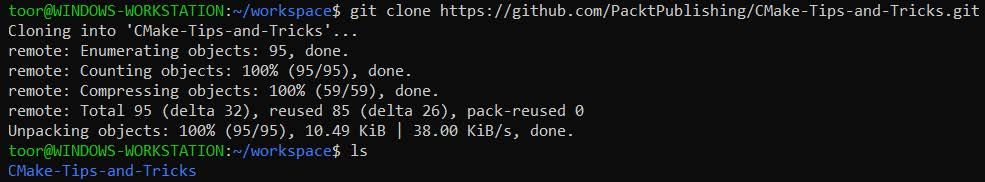
\includegraphics[width=1.\textwidth]{content/1/chapter2/images/3.jpg}\\
Figure 2.3 – Cloning the example code repository
\end{center}

\begin{tcolorbox}[colback=webgreen!5!white,colframe=webgreen!75!black,title=Important Note]
The project must be already present in your environment. If not, clone it via Git by issuing git clone \url{https://github.com/PacktPublishing/CMake-Best-Practices.git} in your terminal.
\end{tcolorbox}

Now go into the CMake-Best-Practices directory and issue cmake -G "Unix Makefiles" -S . -B ./build, as shown in the following figure:

\begin{center}
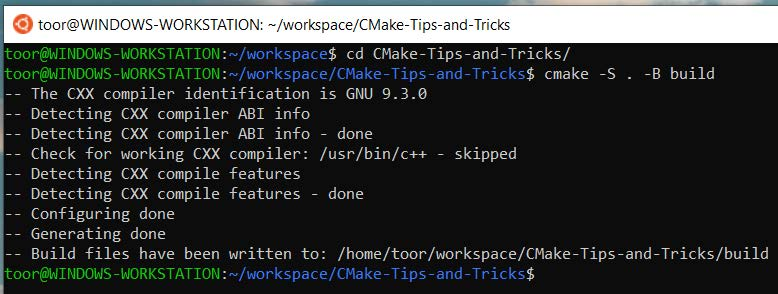
\includegraphics[width=1.\textwidth]{content/1/chapter2/images/4.jpg}\\
Figure 2.4 – Configuring the example code with CMake
\end{center}

This command is like saying to CMake, Use the "Unix Makefiles" (-G "Unix Makefiles") generator to generate a build system for the CMake project in the current directory (-S .) to build (-B ./build) directory.

CMake will configure the project located in the current folder in the build folder. As we omitted the build type, CMake used the Debug build type (the default CMAKE\_BUILD\_TYPE value for the project).

In subsequent sections, we are going to learn about the fundamental settings that are used in the configure step.

\hspace*{\fill} \\ %插入空行
\noindent
\textbf{Changing the build type}

CMake does not assume any build type by default. In order to set the build type, an additional variable named CMAKE\_BUILD\_TYPE must be supplied to the configure command. To supply additional variables, the variable must be prefixed with -D.

To get the Release build instead of Debug, add the CMAKE\_BUILD\_TYPE variable in the configure command, as mentioned previously: cmake -G "Unix Makefiles" -DCMAKE\_BUILD\_TYPE:STRING=Release -S . -B ./build.

\begin{tcolorbox}[colback=webgreen!5!white,colframe=webgreen!75!black,title=Note]
The CMAKE\_BUILD\_TYPE variable only makes sense for singleconfiguration generators, such as Unix Makefiles and Ninja. In multipleconfiguration generators, such as Visual Studio, the build type is a build-time parameter instead of a configuration-time parameter, thus, it cannot be configured by using the CMAKE\_BUILD\_TYPE parameter.
\end{tcolorbox}

\hspace*{\fill} \\ %插入空行
\noindent
\textbf{Changing the generator type}

Depending on the environment, CMake attempts to select an appropriate generator by default. To specify a generator explicitly, the -G argument must be supplied with a valid generator name. For example, if you want to use Ninja as a build system instead of make, you can change it as follows:

\begin{tcblisting}{commandshell={}}
cmake -G "Ninja" -DCMAKE_BUILD_TYPE:STRING=Debug -S . -B ./
build
\end{tcblisting}

The output should be similar to the command output shown in the following figure:

\begin{center}
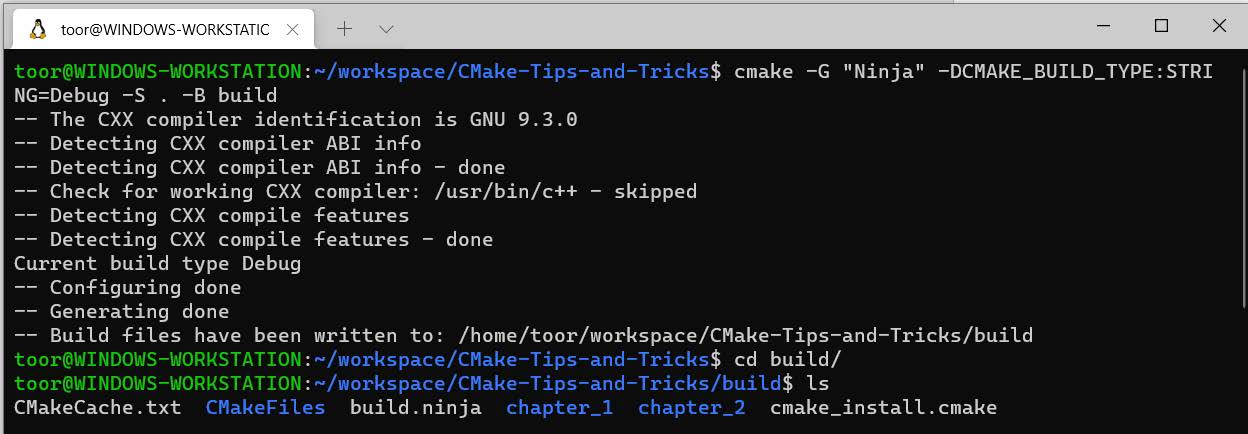
\includegraphics[width=1.\textwidth]{content/1/chapter2/images/5.jpg}\\
Figure 2.5 – Checking the CMake's Ninja generator output
\end{center}

This will cause CMake to generate Ninja build files instead of makefiles.

In order to see all available generator types for your environment, issue the cmake -{}-help command. Available generators will be listed at the end of the Help text generators section, as shown here:

\begin{center}
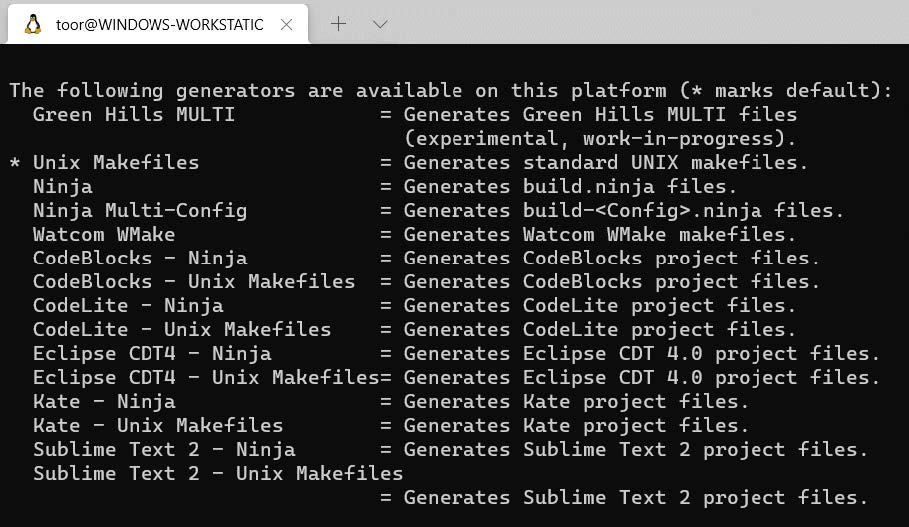
\includegraphics[width=1.\textwidth]{content/1/chapter2/images/6.jpg}\\
Figure 2.6 – List of available generators in help
\end{center}

The generator with one asterisk next to it is the default for the environment you're currently in.

\hspace*{\fill} \\ %插入空行
\noindent
\textbf{Changing the compiler}

In CMake, the compilers to be used are specified on a per-language basis via the CMAKE\_<LANG>\_COMPILER variables. In order to change the compiler for a language, CMAKE\_<LANG>\_COMPILER must be supplied to the Configure command. For a C/C++ project, the variables usually overridden are CMAKE\_C\_COMPILER (C compiler) and CMAKE\_CXX\_COMPILER (C++ compiler). Compiler flags are similarly controlled by the CMAKE\_<LANG>\_FLAGS variable. This variable can be used for holding configuration-independent compiler flags.

As an example, let's try to use g++-10 as a C++ compiler in an environment where it is not the default compiler:

\begin{tcblisting}{commandshell={}}
cmake -G "Unix Makefiles" -DCMAKE_CXX_COMPILER=/usr/bin/g++-10 -S .  
  -B ./build
\end{tcblisting}

Here, we can see g++-10 is used instead of the system's default compiler, g++-9:

\begin{center}
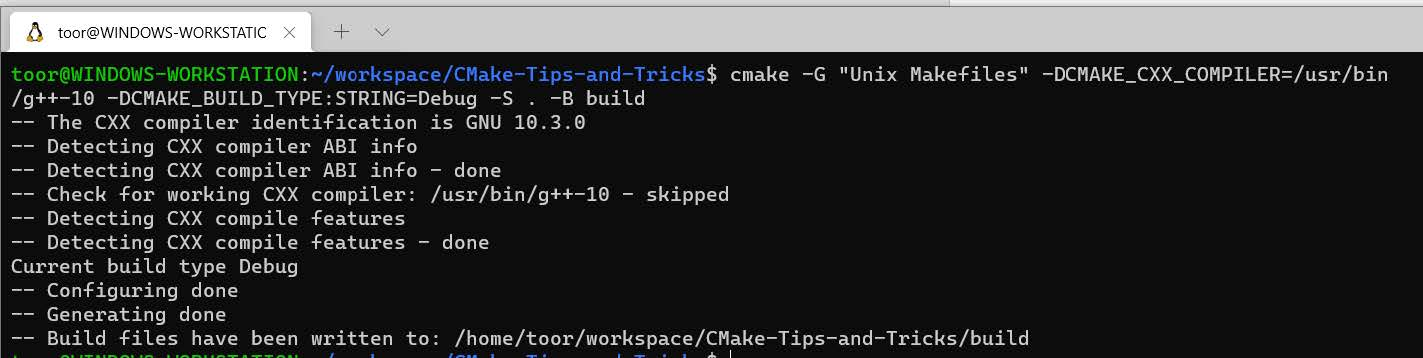
\includegraphics[width=1.\textwidth]{content/1/chapter2/images/7.jpg}\\
Figure 2.7 – Configuring the project using a different compiler (g++-10)
\end{center}

Without the compiler specification, CMake prefers to use g++-9 in this environment:

\begin{center}
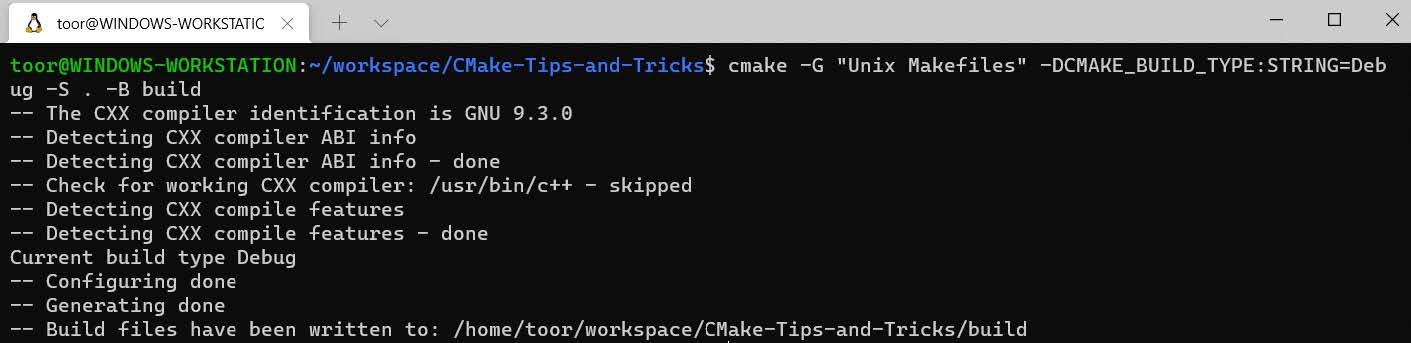
\includegraphics[width=1.\textwidth]{content/1/chapter2/images/8.jpg}\\
Figure 2.8 – Configuring behavior without a compiler preference
\end{center}

\hspace*{\fill} \\ %插入空行
\noindent
\textbf{Passing flags to the compiler}

To illustrate how to specify compiler flags, suppose that you want to enable all warnings and treat them as an error. These behaviors are controlled with -Wall and -Werror compiler flags, respectively, in the gcc toolchain; thus, we need to pass these flags to the C++ compiler. The following code specifies how to do it:

\begin{tcblisting}{commandshell={}}
cmake -G "Unix Makefiles" -DCMAKE_CXX_FLAGS:STRING="-Wall
  -Werror" - S . B ./build S . -B ./build
\end{tcblisting}

We can see the flags specified in the command (-Wall and -Werror) are passed into the compiler in the following example:

\begin{center}
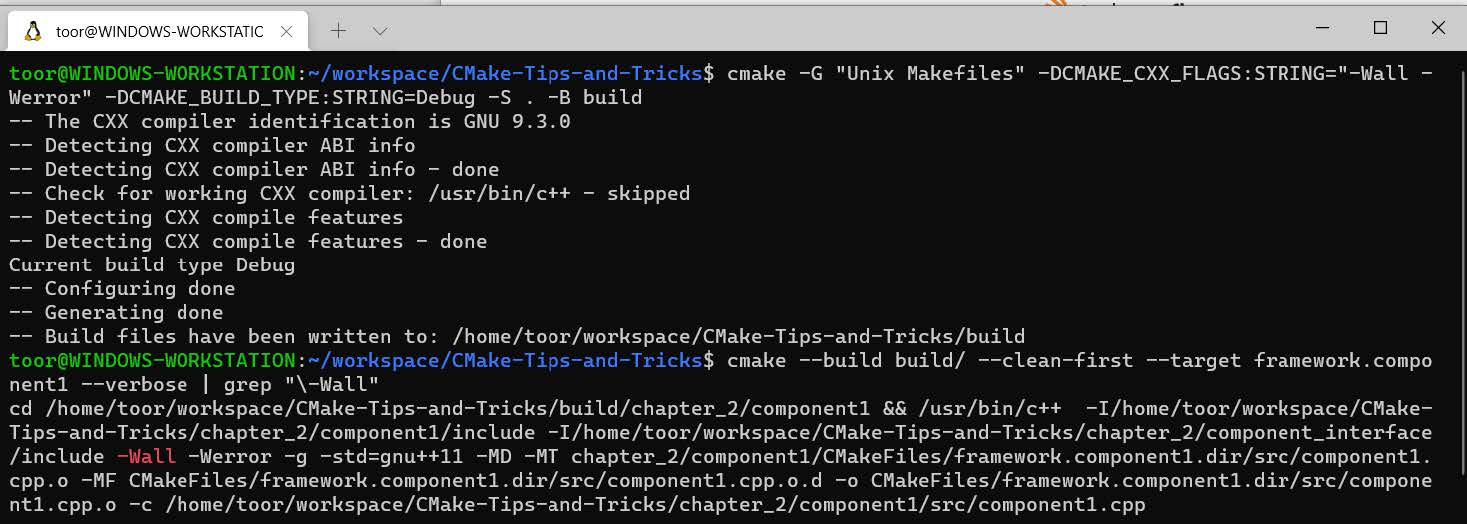
\includegraphics[width=1.\textwidth]{content/1/chapter2/images/9.jpg}\\
Figure 2.9 – Passing flags to the C++ compiler
\end{center}

Build flags can be customized for a per-build type by suffixing them with capitalized build type string. There are four variables for four  different build types, as listed next. They are useful for specifying build types depending on compiler flags. Flags specified in such variables are only valid when the configuration build type matches:











